\documentclass[11pt]{article}

\usepackage[utf8]{inputenc}
\usepackage[T1]{fontenc}
\usepackage{amsmath,amssymb,amsthm}
\usepackage{graphicx}
\usepackage{geometry}
\usepackage{hyperref}
\usepackage{booktabs}
\usepackage{array}
\usepackage{cite}
\usepackage{xcolor}
\usepackage{mathtools}

\geometry{margin=1in}

\title{Drosophila Dual-Goal Steering Dynamics}
\author{Melissa Tian, Tim Lin}
\date{May 12th, 2026}

\begin{document}

\maketitle

\hrule
\vspace{1em}

\section{Introduction}

Goal-directed navigation requires transforming allocentric spatial representations into egocentric motor commands. In \textit{Drosophila}, the central complex implements this transformation through a well-characterized circuit connecting the head direction system to descending motor neurons \cite{westeinde2024}. Three PFL neuron populations --- PFL3R, PFL3L, and PFL2 --- receive shifted copies of the head direction vector (phase shifts of $+67.5^\circ$, $-67.5^\circ$, and $180^\circ$ respectively) and compare these with a goal vector represented in the fan-shaped body. Each cell sums its heading input with the goal input, passes the sum through a nonlinearity, and projects onto the descending neurons DNa02 and DNa03 that ultimately drive steering. The full circuit, as characterized by Westeinde et al. \cite{westeinde2024}, implements a model of the steering system where the steering drive $U(\theta)$ is represented by

\begin{align}
U(\theta) & =f\left( \sum g_{PFL3L}+W_{DNa03}\cdot f\left( \sum g_{PFL3L}+\sum g_{PFL2L} \right) \right) \notag \\
 & \quad -f\left( \sum g_{PFL3R}+W_{DNa03}\cdot f\left( \sum g_{PFL3R}+\sum g_{PFL2R} \right) \right)
\end{align}

This biological circuit-based model contains a direct pathway (PFL3 $\to$ DNa02) with an indirect pathway (PFL3, PFL2 $\to$ DNa03 $\to$ DNa02) in which PFL2 cells provide adaptive gain control. The resulting rotational velocity $\dot\theta \propto U(\theta)$ varies sinusoidally with directional error and produces a single stable fixed point at the goal.

This elegant architecture raises a natural question: \textbf{what happens when the fly must navigate in the face of two simultaneous / competing goals?} This project investigates how the nonlinear structure of the PFL circuit, upon receiving two simultaneous goal headings, can generate a double-well potential in heading space, and derives conditions under which the resulting dynamics approximate the forced Duffing oscillator --- a canonical model for chaos and complex oscillations in nonlinear systems \cite{guckenheimer1983}.

To do so, in \textbf{Section 2}, we (i) extend the goal representation in eq. ($*$) to a sum of two von Mises bumps at $\pm\delta$, modeling two simultaneously presented goals; (ii) specialize the per-cell nonlinearity to $f(x) = x^2$, which permits an exact closed-form evaluation of the population integrals; and (iii) consider the simplified circuit in which PFL2 input is removed. Under these assumptions, the steering signal $U(\theta, \delta)$ can be derived analytically. A local Taylor expansion of $U(\theta, \delta)$ around $\theta = 0$ truncated at cubic order produces $\dot\theta \approx A(\delta, \kappa)\theta - B(\delta, \kappa)\theta^3$, the right-hand side of a Duffing oscillator.

With the reduced system constructed, in \textbf{Section 3}, we first establish that this system undergoes a supercritical pitchfork bifurcation. Promoting the dynamics to second order by adding inertia and damping, we the examined its phase portrait and identified its difference with the system before truncation. Finally, in \textbf{Section 4}, when the system undergoes periodic forcing, we characterize the onset of chaos using Melnikov's method and verify the prediction numerically.

The Duffing reduction therefore serves as both a tractable analytical model of the \textit{Drosophila} dual-goal steering dynamics and a useful diagnostic of where neural-circuit dynamics share features with this well-characterized classic nonlinear system. The validity of the local reduction, and where it breaks down in the full $S^1$ space, is a recurring theme throughout the report.

\section{Derivation of the Reduced System}

\subsection{Analytical Form of the Steering Drive}

Taking a reference frame where the two goals, $\theta_{\text{goal}}^{(0)}$ and $\theta_{\text{goal}}^{(1)}$, are located at $\delta$ and $-\delta$ respectively, we can write the von Mises bump representation, under this dual-goal, for a goal neuron with preference $\phi$ as:

\begin{equation}
g_{\text{goal}}(\phi, \delta) = \exp(\kappa_{\text{goal}} \cos(\delta - \phi)) + \exp(\kappa_{\text{goal}} \cos(-\delta - \phi))
\end{equation}

similarly write down the heading neurons with preference $\phi$ firing to the current heading $\theta$ as:

\begin{equation}
g_{\text{heading}}(\phi, \theta) = \exp(\kappa_{\text{heading}} \cos(\theta - \phi))
\end{equation}

Considering a PFL cell with goal preference $\phi$, we abstract that each cell receives a direct synaptic connection from the associated goal neuron, as well as a synaptic connection from a heading neuron tuned to $\Delta_{\text{pop}}$ away from $\phi$. Showing the PFL3L subpopulation as an example, we can write down the total drive to a PFL3L neuron with preference $\phi$, $h_{PFL3}$, and the neural activity after the nonlinearity $f$, $g_{PFL3}$, as:

\begin{equation}
\begin{aligned}
h_{PFL3L}(\theta, \phi, \delta) &= S \cdot g_{\text{heading}}(\phi - \Delta_{PFL3}, \theta) + A \cdot g_{\text{goal}}(\phi, \delta) \\
&= S \cdot \exp(\kappa_{\text{heading}} \cos(\theta - (\phi - \Delta_{PFL3}))) \\
&\quad + A \cdot (\exp(\kappa_{\text{goal}} \cos(\delta - \phi)) + \exp(\kappa_{\text{goal}} \cos(-\delta - \phi))) \\
g_{PFL3L}(\theta, \phi, \delta) &= f(h_{PFL3}(\theta, \phi, \delta))
\end{aligned}
\end{equation}

As downstream neurons to the PFLs (DNa02 and DNa03) effectively sum inputs from all neurons of each population (PFL3L/R, PFL2), it behooves us to consider the population activity as a whole, integrating eq. (3) over all $\phi$. We can write down the population activity of the PFL3L subpopulation:

\begin{equation}
\begin{aligned}
G_{PFL3L}(\theta, \delta) &= \int_{-\pi}^{\pi} g_{PFL3L}(\theta, \phi, \delta)\, d\phi \\
&= \int_{-\pi}^{\pi} f(h_{PFL3L}(\theta, \phi, \delta))\, d\phi
\end{aligned}
\end{equation}

We choose the quadratic nonlinearity $f(x) = x^2$, as a precedented choice in neuroscience and one that allows conjunctive tuning for heading and goal states on the level of PFL3 neurons \cite{hennequin2018}. This is important to allow differences between the L and R populations after integration.

Hence we have the following:

\begin{equation}
\begin{aligned}
G_{PFL3L}(\theta, \delta) &= \int_{-\pi}^{\pi} h_{PFL3}(\theta, \phi, \delta)^2 \, d\phi \\
&= \int_{-\pi}^{\pi} (S \cdot g_{\text{heading}}(\phi - \Delta_{PFL3}, \theta) + A \cdot g_{\text{goal}}(\phi, \delta))^2 \, d\phi \\
&= \int_{-\pi}^{\pi} \big[ S^2 \cdot g_{\text{heading}}(\phi - \Delta_{PFL3}, \theta)^2 + A^2 \cdot g_{\text{goal}}(\phi, \delta)^2 \\
&\quad + 2SA \cdot g_{\text{heading}}(\phi - \Delta_{PFL3}, \theta) \cdot g_{\text{goal}}(\phi, \delta) \big] d\phi
\end{aligned}
\end{equation}

As $\int_{-\pi}^{\pi} g_{\text{heading}}(\phi - \Delta_{PFL3}, \theta)^2 \, d\phi = \int_{-\pi}^{\pi} g_{\text{heading}}(\phi + \Delta_{PFL3}, \theta)^2 \, d\phi$, we can simplify the difference in population activity between the PFL3L and PFL3R subpopulations as:

\begin{equation}
\begin{aligned}
G_{PFL3L}(\theta, \delta) - G_{PFL3R}(\theta, \delta) &= 2SA \int_{-\pi}^{\pi} \big( g_{\text{heading}}(\phi - \Delta_{PFL3}, \theta) - g_{\text{heading}}(\phi + \Delta_{PFL3}, \theta) \big) g_{\text{goal}}(\phi, \delta)\, d\phi \\
&= 2SA \int_{-\pi}^{\pi} \big( \exp(\kappa_{\text{heading}} \cos(\theta - (\phi - \Delta_{PFL3}))) \\
&\quad - \exp(\kappa_{\text{heading}} \cos(\theta - (\phi + \Delta_{PFL3}))) \big) \\
&\quad \cdot \big( \exp(\kappa_{\text{goal}} \cos(\delta - \phi)) + \exp(\kappa_{\text{goal}} \cos(-\delta - \phi)) \big) d\phi
\end{aligned}
\end{equation}

Let $\xi_\phi(a, b): S^1 \times S^1 \to \mathbb{R} = \exp(\kappa_{\text{heading}} \cos(a - \phi) + \kappa_{\text{goal}} \cos(b - \phi))$, we can rewrite the above as:

\begin{equation}
\begin{aligned}
G_{PFL3L}(\theta, \delta) - G_{PFL3R}(\theta, \delta) = 2SA \int_{-\pi}^{\pi} \big( &\xi_\phi(\theta + \Delta_{PFL3}, \delta) + \xi_\phi(\theta + \Delta_{PFL3}, -\delta) \\
- &\xi_\phi(\theta - \Delta_{PFL3}, \delta) - \xi_\phi(\theta - \Delta_{PFL3}, -\delta) \big) d\phi
\end{aligned}
\end{equation}

Noting that:

\begin{equation*}
\kappa_{\text{heading}} \cos(\phi - a) + \kappa_{\text{goal}} \cos(\phi - b) = \kappa(a, b) \cos(\phi - \mu(a,b))
\end{equation*}

where the effective concentration is

\begin{equation*}
\kappa(a, b) = \sqrt{\kappa_{\text{heading}}^2 + \kappa_{\text{goal}}^2 + 2\kappa_{\text{heading}}\kappa_{\text{goal}} \cos(a - b)}
\end{equation*}

and the effective phase is

\begin{equation*}
\mu(a, b) = \operatorname{atan2}\big(\kappa_{\text{heading}}\sin a + \kappa_{\text{goal}}\sin b,\; \kappa_{\text{heading}}\cos a + \kappa_{\text{goal}}\cos b\big).
\end{equation*}

This is the standard phasor sum: two cosines with the same argument variable $\phi$ but different phases $a, b$ combine into a single cosine with concentration $\kappa(a,b)$ and phase $\mu(a,b)$. Note that $\mu$ depends on $a, b$ but, crucially, drops out after integration over the full period in $\phi$ (see below).

We can evaluate each piece of the integral as:

\begin{equation}
\begin{aligned}
\int_{-\pi}^{\pi} \xi_\phi(a, b)\, d\phi &= \int_{-\pi}^{\pi} \exp(\kappa_{\text{heading}} \cos(a - \phi) + \kappa_{\text{goal}} \cos(b - \phi))\, d\phi \\
&= \int_{-\pi}^{\pi} \exp(\kappa(a, b) \cos(\phi - \mu(a,b)))\, d\phi \\
&= 2\pi I_0(\kappa(a, b))
\end{aligned}
\end{equation}

The last equality uses the standard identity $\int_{-\pi}^{\pi} \exp(\kappa \cos(\phi - \mu))\, d\phi = 2\pi I_0(\kappa)$, which is independent of $\mu$ by translation invariance of the integration measure on $S^1$. Here $I_0$ is the modified Bessel function of the first kind, order 0.

Hence we have the following closed form solution for the difference in population activity between the PFL3L and PFL3R subpopulations:

\begin{equation}
\begin{aligned}
G_{PFL3L}(\theta, \delta) - G_{PFL3R}(\theta, \delta) = 4\pi SA \big( &I_0(\kappa(\theta + \Delta_{PFL3}, \delta)) + I_0(\kappa(\theta + \Delta_{PFL3}, -\delta)) \\
- &I_0(\kappa(\theta - \Delta_{PFL3}, \delta)) - I_0(\kappa(\theta - \Delta_{PFL3}, -\delta)) \big)
\end{aligned}
\end{equation}

Now, in the simplified system where there is no PFL2 input and the DNa02s and DNa03s simply sum the PFL3L and PFL3R population activity respectively, we can write down the steering drive as:

\begin{equation}
U(\theta, \delta) = G_{PFL3}(\theta, \delta) - G_{PFL3R}(\theta, \delta)
\end{equation}

This form of $U$ will be referred to as the \textbf{Bessel model} in the following text and figures.

Numerical calculation from the Bessel model, the discrete PFL3 model with 12 neurons on each side (corresponding to the biological circuit), and the full circuit model (with PFL2 neurons considered) yield very similarly shaped $U(\theta)$, supporting the validity of our simplifications. For the following analysis, we will continue with the PFL3 only circuit, using the 12 neuron discrete model as the ground-truth comparison.

\begin{figure}[h]
\centering
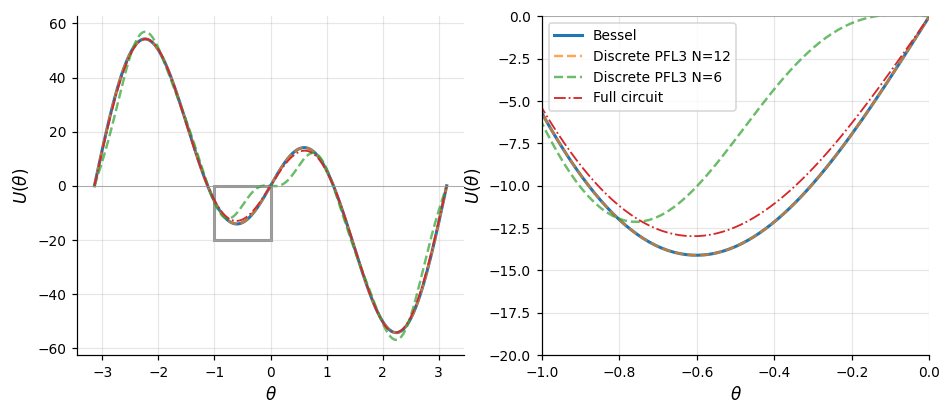
\includegraphics[width=0.85\textwidth]{figures/fig1.png}
\caption{Steering drive $U(\theta)$ from different models.}
\end{figure}

\subsection{Taylor Expansion Approximation of the Steering Drive}

\subsubsection{Symmetry of $U(\theta, \delta)$}

Before computing the Taylor expansion, we record two symmetry properties that will simplify the derivatives at $\theta = 0$.

\textbf{Property (a): $\kappa(a, b)$ depends on $a, b$ only through $\cos(a - b)$.} Direct from the definition of $\kappa(a,b)$.

\textbf{Property (b): $U$ is odd in $\theta$ at fixed $\delta$.} Apply the substitution $\theta \to -\theta$ to the four arguments in eq. (9):

\begin{center}
\begin{tabular}{ll}
\toprule
Original & After $\theta \to -\theta$ \\
\midrule
$\kappa(\theta + \Delta_{PFL3}, \delta)$  & $\kappa(-\theta + \Delta_{PFL3}, \delta)$  \\
$\kappa(\theta + \Delta_{PFL3}, -\delta)$ & $\kappa(-\theta + \Delta_{PFL3}, -\delta)$ \\
$\kappa(\theta - \Delta_{PFL3}, \delta)$  & $\kappa(-\theta - \Delta_{PFL3}, \delta)$  \\
$\kappa(\theta - \Delta_{PFL3}, -\delta)$ & $\kappa(-\theta - \Delta_{PFL3}, -\delta)$ \\
\bottomrule
\end{tabular}
\end{center}

Using property (a) --- that $\kappa$ depends on the \textit{difference} of its arguments via cosine --- we have $\kappa(-\theta + \Delta_{PFL3}, \delta) = \kappa(\theta - \Delta_{PFL3}, -\delta)$ (both have $\cos$ of $-\theta + \Delta_{PFL3} - \delta$ inside). Working through all four, the four terms after $\theta \to -\theta$ are precisely the four original terms with their signs swapped. Therefore

\begin{equation*}
U(-\theta, \delta) = -U(\theta, \delta),
\end{equation*}

i.e. $U$ is odd in $\theta$. As corollaries:

\begin{itemize}
\item $U(0, \delta) = 0$ for all $\delta$.
\item All even-order derivatives vanish at $\theta = 0$: $U^{(2k)}(0, \delta) = 0$.
\end{itemize}

This is the systematic version of ``the function is odd around $\theta = 0$'' used below.

\subsubsection{Taylor expansion of $U(\theta, \delta)$ around $\theta = 0$}

We expand $U(\theta, \delta)$ around $\theta = 0$ for our dreamed Duffing connection:

\begin{equation}
U(\theta, \delta) = U(0, \delta) + U'(0, \delta)\,\theta + \frac{1}{2} U''(0, \delta)\,\theta^2 + \frac{1}{6} U'''(0, \delta)\,\theta^3 + O(\theta^4)
\end{equation}

By the symmetry result of §1.1:

\begin{equation}
U(0, \delta) = 0, \qquad U''(0, \delta) = 0.
\end{equation}

Only the odd-order terms survive at this order, giving the Duffing-form

\begin{equation*}
U(\theta, \delta) \approx U'(0, \delta)\,\theta + \frac{1}{6} U'''(0, \delta)\,\theta^3 + O(\theta^5).
\end{equation*}

\subsubsection{First-order coefficient}

Define $K(\theta; a, b) \equiv \kappa(\theta + a, b)$. By the chain rule:

\begin{equation}
\frac{d}{d\theta} I_0(K(\theta; a, b)) = I_0'(K) \cdot \frac{dK}{d\theta} = I_1(K) \cdot \frac{dK}{d\theta}, \tag{13a}
\end{equation}

using the identity $I_0'(x) = I_1(x)$. The derivative of $K$ is computed from $K^2 = \kappa_h^2 + \kappa_g^2 + 2\kappa_h\kappa_g\cos(\theta + a - b)$, giving $2K K' = -2\kappa_h\kappa_g\sin(\theta + a - b)$, hence

\begin{equation}
\frac{dK}{d\theta} = -\frac{\kappa_h\kappa_g \sin(\theta + a - b)}{K(\theta; a, b)}. \tag{13b}
\end{equation}

Combining:

\begin{equation}
\frac{d}{d\theta} I_0(K(\theta; a, b)) = -I_1(K) \cdot \frac{\kappa_h\kappa_g \sin(\theta + a - b)}{K}. \tag{13c}
\end{equation}

Applying this to each of the four terms in eq. (9) and evaluating at $\theta = 0$:

\begin{equation}
\begin{aligned}
U'(0, \delta) = -4\pi SA\, \kappa_h\kappa_g \bigg[ &\frac{I_1(\kappa(\Delta_{PFL3}, \delta))}{\kappa(\Delta_{PFL3}, \delta)} \sin(\Delta_{PFL3} - \delta) \\
+\, &\frac{I_1(\kappa(\Delta_{PFL3}, -\delta))}{\kappa(\Delta_{PFL3}, -\delta)} \sin(\Delta_{PFL3} + \delta) \\
-\, &\frac{I_1(\kappa(-\Delta_{PFL3}, \delta))}{\kappa(-\Delta_{PFL3}, \delta)} \sin(-\Delta_{PFL3} - \delta) \\
-\, &\frac{I_1(\kappa(-\Delta_{PFL3}, -\delta))}{\kappa(-\Delta_{PFL3}, -\delta)} \sin(-\Delta_{PFL3} + \delta) \bigg].
\end{aligned}
\end{equation}

Using $\kappa(-\Delta_{PFL3}, \delta) = \kappa(\Delta_{PFL3}, -\delta)$ and $\kappa(-\Delta_{PFL3}, -\delta) = \kappa(\Delta_{PFL3}, \delta)$ (property (a)), and $\sin(-x) = -\sin(x)$, the four terms collapse pairwise:

\begin{equation}
\boxed{\;U'(0, \delta) = -8\pi SA\, \kappa_h\kappa_g \left[ \frac{I_1(\kappa(\Delta_{PFL3}, \delta))}{\kappa(\Delta_{PFL3}, \delta)} \sin(\Delta_{PFL3} - \delta) + \frac{I_1(\kappa(\Delta_{PFL3}, -\delta))}{\kappa(\Delta_{PFL3}, -\delta)} \sin(\Delta_{PFL3} + \delta) \right]\;}
\end{equation}

\subsubsection{Third-order coefficient}

We need $\frac{d^3}{d\theta^3} I_0(K(\theta; a, b))$ at $\theta = 0$, with derivatives $K', K'', K'''$ taken with respect to $\theta$. From $K^2 = \kappa_h^2 + \kappa_g^2 + 2\kappa_h\kappa_g\cos(\theta + a - b)$, define

\begin{equation*}
C(\theta) \equiv \kappa_h\kappa_g\cos(\theta + a - b), \qquad S(\theta) \equiv \kappa_h\kappa_g\sin(\theta + a - b).
\end{equation*}

Then $K^2 = \kappa_h^2 + \kappa_g^2 + 2C$, and successive differentiation gives:

\begin{equation*}
\begin{aligned}
K' &= -\frac{S}{K} \\
K'' &= -\frac{C}{K} - \frac{(K')^2}{K} = -\frac{C}{K} - \frac{S^2}{K^3} \\
K''' &= \frac{d}{d\theta}\left[ -\frac{C}{K} \right]+\frac{d}{d\theta}\left[ -\frac{S^{2}}{K^{3}} \right]=\frac{S}{K}-\frac{CS}{K^{3}}-\frac{2SC}{K^{3}}-\frac{3S^{3}}{K^{5}}=\frac{S}{K}-\frac{3SC}{K^{3}}-\frac{3S^{3}}{K^{5}}
\end{aligned}
\end{equation*}

For the Bessel side, use the recurrences $I_0' = I_1$, $I_1' = \tfrac{1}{2}(I_0 + I_2)$, $I_1'' = \tfrac{1}{4}(3I_1 + I_3)$.

Applying the chain rule three times:

\begin{align*}
I_{0}' & =I_{1}\\
I_{0}'' & =I_{1}'=\frac{1}{2}[I_{0}(x)+I_{2}(x)] \\
I_{0}'''& =I_{1}''=\frac{1}{2}[I_{0}(x)+I_{2}(x)]'=\frac{1}{2}\left[ I_{1}(x)+\frac{1}{2}(I_{1})(x)+I_{3}(x) \right]=\frac{1}{4}[3I_{1}(x)+I_{3}(x)]
\end{align*}

Taken together, we have

\begin{align*}
\frac{d^3}{d\theta^3} I_0(K) & = I_0'''(K) (K')^3 + 3 I_0''(K) K' K'' + I_0'(K) K'''  \\
 & = \frac{1}{4}[3I_{1}(K)+I_{3}(K)] \cdot\left( -\frac{S^{3}}{K^{3}} \right)\\
  & \quad + \underbrace{3 \cdot \frac{1}{2}[I_0(K) + I_2(K)] \cdot \left(\frac{SC}{K^2} + \frac{S^3}{K^4}\right)}_{\text{from } 3 I_0''(K) K' K''} \\
   & \quad +\underbrace{I_1(K) \cdot \left(\frac{S}{K} - \frac{3CS}{K^3} - \frac{3 S^3}{K^5}\right)}_{\text{from } I_0'(K) K'''}
\end{align*}

With $\frac{d^3}{d\theta^3} I_0(K)$ in hand, the third-order coefficient of $U$ is the sum over the four arguments of eq. (9):

\begin{equation}
U'''(0, \delta) = 4\pi SA \sum_{(a, b) \in \mathcal{P}} \sigma(a) \cdot \frac{d^3}{d\theta^3} I_0(K(\theta; a, b)) \bigg|_{\theta = 0}
\end{equation}

where $\mathcal{P} = \{(\Delta_{PFL3}, \delta), (\Delta_{PFL3}, -\delta), (-\Delta_{PFL3}, \delta), (-\Delta_{PFL3}, -\delta)\}$ and $\sigma(a) = +1$ for $a = +\Delta_{PFL3}$, $-1$ for $a = -\Delta_{PFL3}$ (matching the signs in eq. 9).

By property (a), the four-term sum simplifies to two terms after pairing, which gives us

\begin{equation}
\boxed{U'''(0, \delta) = 8\pi SA\kappa_{h}\kappa_{g}[\sin(\Delta_{PFL3}-\delta)\cdot D(\kappa_{-},C_{-},S_{-})+\sin (\Delta_{P_{3}L}+\delta)\cdot D(\kappa_{+},C_{+},S_{+})]}
\end{equation}

with
\begin{align*}
D(K,C,S) & =\frac{1}{K}\bigl[ I_{1}(K)\left( 1-\frac{3C}{K^{2}}-\frac{3S^{2}}{K^{4}} \right)+\frac{3(I_{0}(K)+I_{2}(K))}{2}\left( \frac{C}{K} + \frac{S^{2}}{K^{3}} \right) \\
 & -\frac{3I_{1}(K)+I_{3}(K)}{4}\cdot \frac{S^{2}}{K^{2}} \bigr]
\end{align*}
and
\begin{align*}
\kappa_- &\equiv \kappa(\Delta_{PFL3}, \delta) = \sqrt{\kappa_h^2 + \kappa_g^2 + 2\kappa_h\kappa_g\cos(\Delta_{PFL3} - \delta)} \\
\kappa_+ &\equiv \kappa(\Delta_{PFL3}, -\delta) = \sqrt{\kappa_h^2 + \kappa_g^2 + 2\kappa_h\kappa_g\cos(\Delta_{PFL3} + \delta)} \\
C_- &\equiv \kappa_h\kappa_g\cos(\Delta_{PFL3} - \delta), \qquad C_+ \equiv \kappa_h\kappa_g\cos(\Delta_{PFL3} + \delta) \\
S_- &\equiv \kappa_h\kappa_g\sin(\Delta_{PFL3} - \delta), \qquad S_+ \equiv \kappa_h\kappa_g\sin(\Delta_{PFL3} + \delta)
\end{align*}

\subsubsection{Local cubic expansion of the steering drive}

Combining §1.3--§1.5, the local expansion of the steering drive is

\begin{equation}
\dot{\theta}=U(\theta, \delta) \approx A(\delta)\,\theta - B(\delta)\,\theta^3 + O(\theta^5),
\end{equation}
with
\begin{equation*}
A(\delta) \equiv U'(0, \delta), \qquad B(\delta) \equiv -\frac{1}{6} U'''(0, \delta).
\end{equation*}
in order the match the conventional expression of the Duffing equation.

\subsection{Body Mechanics and Second-Order Dynamics}

Consider the fly as a rigid body with rotational inertia $I$ and rotational drag $\gamma$.

The reduction up to §1.2.5 yields a \textbf{first-order} equation, in which the circuit's output is interpreted (following Westeinde et al.) as a direct angular-velocity command. This is the natural overdamped limit of the fly's heading dynamics: velocity is directly proportional to the steering signal with no inertial transients.

If we restore the inertia term and instead interpret the steering signal $U(\theta,\delta)$ as a \textbf{torque command} rather than a angular velocity command, Newton's second law for then gives

\begin{equation}
I \ddot{\theta} + \gamma \dot{\theta} = U(\theta,\delta),
\end{equation}

This contains the first-order model as the overdamped limit $I \to 0$: when inertia is negligible relative to drag, $\ddot\theta$ drops out and one recovers $\gamma\dot\theta = U$.

We note that this is a modeling reinterpretation, not a derivation: the same $U(\theta, \delta)$ that previously carried units of velocity now carries units of torque. The constants $I, \gamma$ enter as phenomenological parameters describing the body dynamics rather than being computed from the circuit itself. An alternative interpretation is that $I$ represents an \textit{effective} inertia arising from circuit and motor lags.

Substituting the local cubic expansion of §1.2.5,

\begin{equation}
I\ddot\theta + \gamma\dot\theta = A(\delta, \kappa)\,\theta - B(\delta, \kappa)\,\theta^3,
\end{equation}

which is the canonical \textbf{unforced double-well Duffing oscillator}.

\section{Equilibrium Structure and Bifurcation Analysis}

\subsection{Supercritical Pitchfork bifurcation and double-well criterion}

The first-order system that we directly derived from the circuit model shares \textbf{equilibrium structure} with the unforced double-well Duffing oscillator $\ddot{\theta}+\gamma \dot{\theta}=A\theta-B\theta^{3}$. In both systems, equilibria are reached at $\theta=0$ and $\theta=\pm \sqrt{ \frac{A}{B} }$ if $\frac{A}{B}>0$.

Linearize at the origin, $\dot{\theta}=A\theta$, so the fixed point at $\theta = 0$ is \textbf{unstable} (i.e., a double-well structure exists in the first-order system) $\text{iff.}\, A(\delta,\kappa) = U'(0, \delta) > 0$. Substituting from eq. (14), the bifurcation curve $A(\delta) = 0$ is given by

\begin{equation*}
-8\pi SA\, \kappa_h\kappa_g \left[ \frac{I_1(\kappa(\Delta_{PFL3}, \delta))}{\kappa(\Delta_{PFL3}, \delta)} \sin(\Delta_{PFL3} - \delta) + \frac{I_1(\kappa(\Delta_{PFL3}, -\delta))}{\kappa(\Delta_{PFL3}, -\delta)} \sin(\Delta_{PFL3} + \delta) \right] =0
\end{equation*}

When in addition $B(\delta,\kappa)>0$ (i.e. $U'''(0,\delta)<0$), two new equilibria emerge at $\theta=\pm \sqrt{ \frac{A}{B} }$, giving the double-well potential structure. Substituting from eq. (17), the condition in which the pitchfork bifurcation is supercritical is given by

\begin{equation*}
8\pi SA\kappa_{h}\kappa_{g}[\sin(\Delta_{PFL3}-\delta)\cdot D(\kappa_{-},C_{-},S_{-})+\sin (\Delta_{P_{3}L}+\delta)\cdot D(\kappa_{+},C_{+},S_{+})]<0
\end{equation*}

These are transcendental equations in $(\delta, \kappa_h, \kappa_g)$ at fixed $\Delta_{PFL3} = 67.5^\circ$, and setting $\kappa_h = \kappa_g \equiv \kappa$ collapses the parameter space to $(\delta, \kappa)$ for presentation. Numerical solutions yield the following bifurcation diagram.

\begin{figure}[h]
\centering
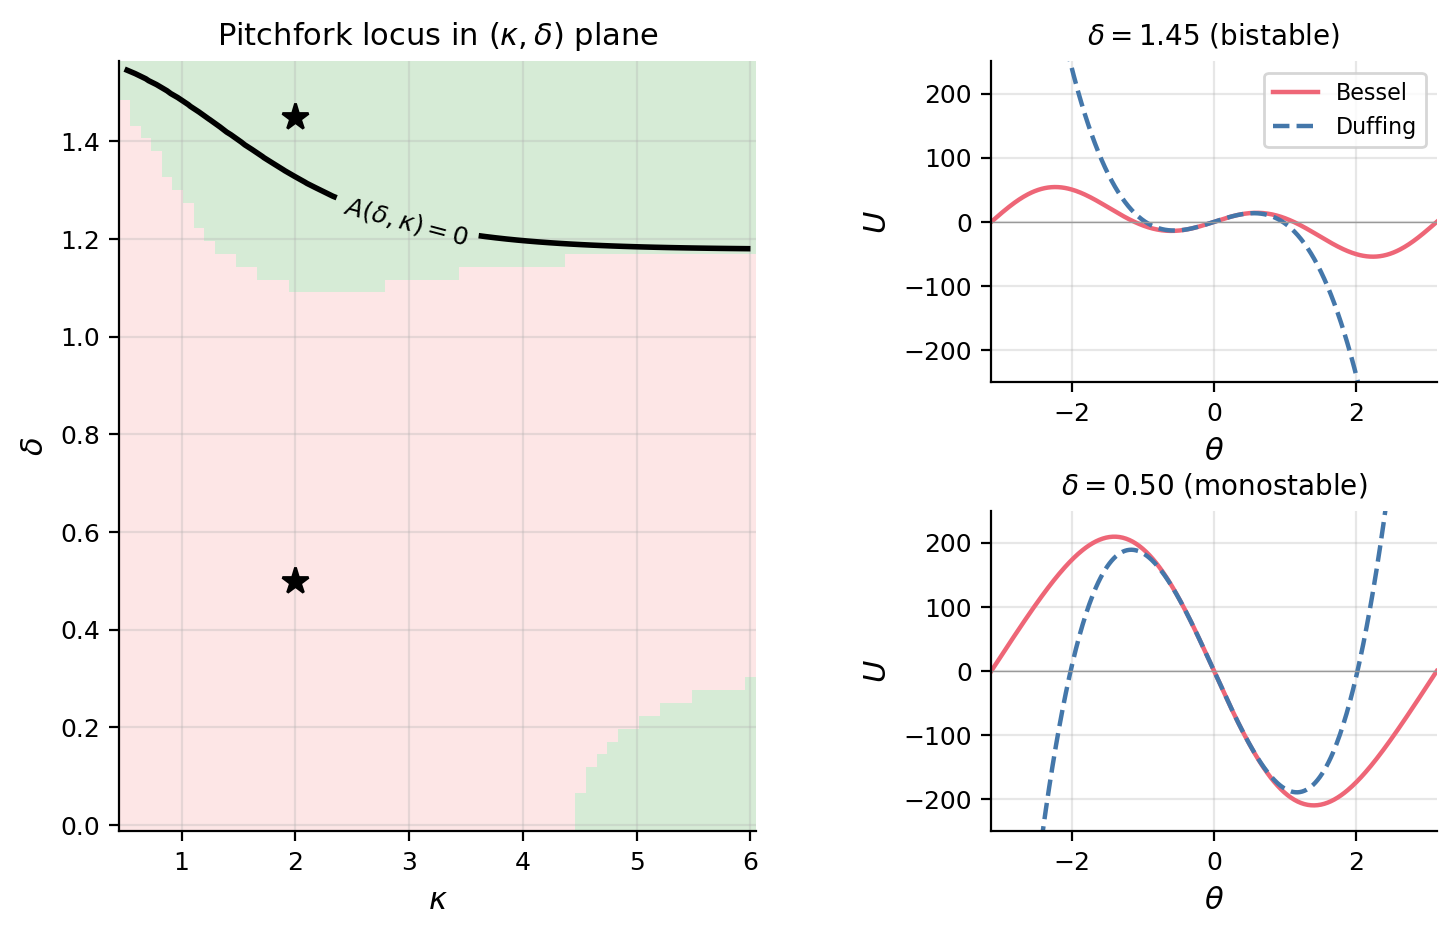
\includegraphics[width=0.85\textwidth]{figures/fig2.png}
\caption{\textbf{Pitchfork bifurcation in $(\kappa,\delta)$ parameter space.} \textbf{Left}, the black curve marks the pitchfork bifurcation curve, where the origin changes stability. Above the curve, $A>0$ and the origin is unstable; below the curve, $A<0$ and the origin is the unique stable fixed point. Green shading indicates where the cubic coefficient $B(\delta,\kappa)>0$, corresponding to a supercritical pitchfork; red shading indicates $B(\delta,\kappa)<0$. \textbf{Right}, the exact steering drive $U(\theta)$ (red, from the Bessel model) with its local Duffing truncation (blue dashed) at two sample parameter points.}
\end{figure}

We can see that the bifurcation boundary lies in the area where $B(\delta,\kappa)>0$ (green shadow), indicating that the bifurcation is a \textbf{supercritical pitchfork} everywhere. This implies the transition from monostable to bistable is smooth --- no jumps or hysteresis as parameters cross the boundary.

The top right panel shows a sample parameter point from the green area above the curve, which is the double-well regime that we are interested in. The approximation is good near $\theta=0$, capturing the saddle and two flanking stable equilibria. At large $\theta$, it diverges from the exact model, where the Bessel curve has additional zero-crossings near $\theta=\pm \pi$ that the Duffing truncation misses entirely. These correspond to fixed points associated with the anti-midpoint of the two goals, which lie outside the local domain of validity of the Taylor expansion. The Duffing reduction therefore is reliable for \textbf{small-amplitude dynamics}, but global features of the $S^{1}$ phase space require the exact steering drive, i.e. the Bessel model.

\subsection{Phase Portrait}

To set up the chaos analysis in Section 4, we first examine the full phase space of the second-order system in its conservative limit ($\gamma=0$). Setting damping to zero in eq. (18) gives:
\begin{equation*}
I \ddot{\theta} = U(\theta,\delta)
\end{equation*}
This system conserves the energy
\begin{equation}
H(\theta,\dot{\theta})=\frac{1}{2}I \dot{\theta}^{2}+V(\theta), \qquad V(\theta)=\int_{0}^{\theta}U(\theta',\delta)d\theta',
\end{equation}

Trajectories lie on level sets of $H$ in the phase plane $(\theta,\dot{\theta})$. Equilibria are zeros of $U(\theta,\delta)$, with stability determined by the sign of $V''(\theta)$.

\begin{figure}[h]
\centering
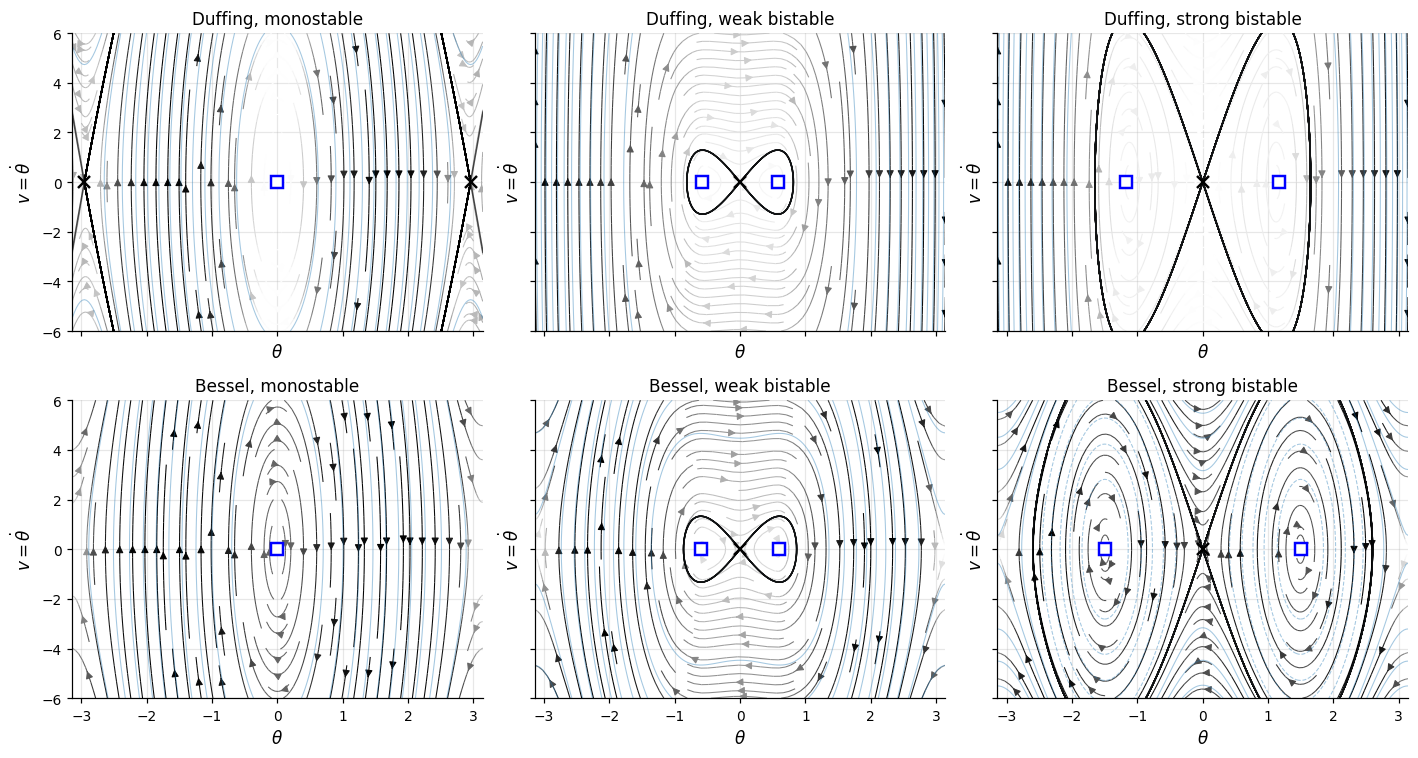
\includegraphics[width=0.85\textwidth]{figures/fig3.png}
\caption{Phase portrait with $\kappa_{g}=\kappa_{h}=2,\delta \in \{ 1,1.36,1.55 \}$. Top row shows the Duffing truncation model, bottom row shows the exact Bessel model. Columns show three parameter regimes on the pitchfork bifurcation curve: mono-stable ($A<0$), week stable (A slightly positive), and strong bistable ($A>0$).}
\end{figure}

In the monostable case, both models exhibit a single center at $\theta = 0$, surrounded by closed orbits that correspond to small-amplitude oscillations around the merged-goal direction. The Duffing truncation's saddles, located at $\theta = \pm\sqrt{|A|/B}$ bound the basin of locally bounded motion; in the exact Bessel system, the corresponding saddles lie near $\theta = \pm\pi$ (the anti-midpoint).

In the weakly bistable case, crossing the pitchfork curve gives rise to the classical figure-eight separatrix structure: two centers at $\theta_\pm = \pm\sqrt{A/B}$ flank a saddle at the origin, joined by \textbf{a pair of homoclinic orbits} that bound the oscillatory motion. The Duffing and Bessel portraits are nearly indistinguishable here. For the remainder of the calculations we work in the weak-bistable regime, where the local approximation is reliable and the canonical Melnikov method applies.

In the strong bistable regime, the two models diverge geometrically. The Duffing truncation continues to predict a closed figure-eight, with the two homoclinic loops expanding as $A$ grows. The exact Bessel system instead shows the saddle's stable and unstable manifolds \textit{escaping} the figure-eight structure: rather than closing back on themselves locally, they extend toward the secondary saddles near $\theta = \pm\pi$. The locally a homoclinic loop becomes globally a \textbf{heteroclinic connection} between the central saddle and the saddles at the anti-midpoint. We will return to this point in §4.4.

\subsection{The homoclinic orbit}

Th unforced, undamped reduced system $\ddot\theta = A\theta - B\theta^3,$ with $A, B > 0$ (the supercritical regime of §3.1). This is a planar Hamiltonian system with conserved energy

\begin{equation}
H(\theta, \dot{\theta}) = \frac{1}{2}\dot{\theta}^2 - \frac{1}{2}A\theta^2 + \frac{1}{4}B\theta^4.
\end{equation}

The zero-energy level set $H = 0$ consists of two homoclinic loops joining the saddle to itself, one in each half-plane. Solving $\frac{1}{2}\dot\theta^2 = \frac{1}{2}A\theta^2 - \frac{1}{4}B\theta^4$ on the right branch yields the closed-form expression for the homoclinic orbit

\begin{equation}
\boxed{\;\theta_0(t) = \sqrt{\frac{2A}{B}}\operatorname{sech}(\sqrt{A}\,t), \qquad v_0(t) = -\sqrt{\frac{2A}{B}}\sqrt{A}\,\operatorname{sech}(\sqrt{A}\,t)\tanh(\sqrt{A}\,t).\;}
\end{equation}

This orbit reaches its apex $\theta_{\max} = \sqrt{2A/B}$ at $t = 0$ and approaches the saddle exponentially as $t \to \pm\infty$ at rate $\sqrt{A}$. The corresponding loop in the left half-plane is obtained by $\theta_0 \to -\theta_0$; the union forms the figure-eight separatrix that divides the phase plane into the two wells (oscillation around either center) and the region of unbounded growth.

\section{Chaotic Behavior Under Periodic Forcing}

\subsection{Damped, forced Duffing oscillator}

We have established that the steering circuit reduced to its local cubic normal form (eq. 19) is the unforced double-well Duffing oscillator, and that the bistable regime is reached through a supercritical pitchfork in $(\delta, \kappa)$ parameter space. We now ask what happens when this system is driven by periodic forcing. The forced system reads

\begin{equation}
\ddot\theta + \gamma\dot\theta = U(\theta, \delta) + F\cos(\omega t),
\end{equation}

where we have set $I = 1$ for notational economy (this fixes a time-scale; all reported frequencies should be read in units of $\sqrt{I^{-1}}$). The forced Duffing oscillator is the canonical example of a low-dimensional smooth system that exhibits Smale-horseshoe chaos for sufficiently strong forcing \cite{guckenheimer1983}. Our goal in this section is: (i) to derive an analytical condition on $(F, \omega, \gamma, \delta, \kappa)$ at which chaotic dynamics first becomes possible in the reduced system, via Melnikov's method, and (ii) to verify this condition numerically in both the reduced (Duffing) and Bessel models. In doing so, we characterize a second, qualitatively distinct chaotic regime that emerges in the global $S^1$ system but is invisible to the local Duffing reduction.

\subsection{The Melnikov criterion}

Following Guckenheimer \& Holmes \cite[§4.5]{guckenheimer1983}, we cast the forced damped system (20) as an $O(\epsilon)$ perturbation of the Hamiltonian system (21):

\begin{equation}
\dot\theta = v, \qquad \dot v = U(\theta, \delta) + \epsilon\bigl[-\gamma v + F\cos\omega t\bigr],
\end{equation}

where for clarity we have written $U(\theta, \delta)$ --- this stands for the local Duffing $A\theta - B\theta^3$, but the entire derivation below carries over to the full Bessel $U$, a point we will exploit in §4.3. To leading order in $\epsilon$, the Melnikov function $M(t_0)$ measures the signed distance between the stable and unstable manifolds of the perturbed saddle (now a hyperbolic periodic orbit of period $2\pi/\omega$ in the extended phase space) at a fixed phase $\omega t_0$ of the forcing cycle. Simple zeros of $M(t_0)$ correspond to transverse intersections of these manifolds, which by the Smale-Birkhoff theorem imply the existence of a Smale horseshoe, hence chaotic dynamics \cite[Theorem 4.5.3]{guckenheimer1983}.

Writing the unperturbed flow as $\mathbf{f}(\mathbf{x}) = (v, U(\theta))^T$ and the perturbation as $\mathbf{g}(\mathbf{x}, t) = (0, -\gamma v + F\cos\omega t)^T$, the Melnikov function takes the following form \cite[§4.5]{guckenheimer1983}:

\begin{equation}
M(t_0) = \int_{-\infty}^{\infty} \mathbf{f}(\boldsymbol{\gamma}_0(\tau)) \wedge \mathbf{g}(\boldsymbol{\gamma}_0(\tau), \tau + t_0)\,d\tau,
\end{equation}

where $\mathbf{f} \wedge \mathbf{g} \equiv f_1 g_2 - f_2 g_1$ is the scalar wedge product in 2D, and $\boldsymbol{\gamma}_0(\tau) = (\theta_0(\tau), v_0(\tau))$ is the unperturbed homoclinic orbit. This formulation has a clean structural consequence for our problem. Expanding the wedge with our specific $\mathbf{f}, \mathbf{g}$:

\begin{equation}
\mathbf{f} \wedge \mathbf{g} = v\bigl[-\gamma v + F\cos\omega t\bigr] - U(\theta)\cdot 0 = -\gamma v^2 + F v\cos\omega t.
\end{equation}

\textbf{The steering drive $U(\theta)$ drops out of the integrand entirely.} It enters the Melnikov function only implicitly, through its role in shaping the homoclinic orbit $\boldsymbol{\gamma}_0(\tau)$ along which the integral is evaluated. The perturbation $\mathbf{g}$ has its first component zero (no forcing or damping on $\dot\theta$), so the wedge picks out only $f_1 g_2 = v\cdot g_2$. The Melnikov formula becomes

\begin{equation}
M(t_0) = -\gamma\int_{-\infty}^{\infty} v_0(\tau)^2\,d\tau + F\int_{-\infty}^{\infty} v_0(\tau)\cos\omega(\tau + t_0)\,d\tau.
\end{equation}

For the Duffing reduction, the orbit (23) is available in closed form and (27) can be evaluated analytically. The damping integral, with $u = \sqrt{A}\,\tau$ and the elementary $\int_{-\infty}^{\infty}\operatorname{sech}^2 u\,\tanh^2 u\,du = 2/3$:

\begin{equation}
D \equiv \int_{-\infty}^{\infty} v_0(\tau)^2\,d\tau = \frac{2A^2}{B}\cdot\frac{1}{\sqrt{A}}\cdot\frac{2}{3} = \frac{4A^{3/2}}{3B}.
\end{equation}

For the forcing integral, expand $\cos\omega(\tau + t_0) = \cos\omega\tau\cos\omega t_0 - \sin\omega\tau\sin\omega t_0$. Since $v_0(\tau)$ is odd in $\tau$, the $\cos\omega\tau$ piece integrates to zero, leaving

\begin{equation*}
\int_{-\infty}^{\infty} v_0(\tau)\cos\omega(\tau + t_0)\,d\tau = -\sin\omega t_0\int_{-\infty}^{\infty} v_0(\tau)\sin\omega\tau\,d\tau.
\end{equation*}

Using the contour identity

\begin{equation*}
\int_{-\infty}^{\infty} \operatorname{sech}(\alpha\tau)\tanh(\alpha\tau)\sin\omega\tau\,d\tau = -\frac{\pi\omega}{\alpha^2}\operatorname{sech}\!\left(\frac{\pi\omega}{2\alpha}\right),
\end{equation*}

derived from summing residues at the poles $\tau = i\pi(n + \tfrac{1}{2})/\alpha$ of $\operatorname{sech}$, with $\alpha = \sqrt{A}$:

\begin{equation}
\int_{-\infty}^{\infty} v_0(\tau)\sin\omega\tau\,d\tau = \pi\omega\sqrt{\frac{2}{B}}\,\operatorname{sech}\!\left(\frac{\pi\omega}{2\sqrt{A}}\right).
\end{equation}

Combining (27)--(29),

\begin{equation}
\boxed{\;M(t_0) = -\frac{4\gamma A^{3/2}}{3B} - F\pi\omega\sqrt{\frac{2}{B}}\,\operatorname{sech}\!\left(\frac{\pi\omega}{2\sqrt{A}}\right)\sin\omega t_0.\;}
\end{equation}

$M(t_0)$ has simple zeros if and only if the amplitude of the sinusoidal part exceeds the damping bias, which yields our Melnikov threshold

\begin{equation}
\boxed{\;F_{\text{crit}}(\omega) = \frac{4\gamma A}{3\pi\omega\sqrt{2B}}\cosh\!\left(\frac{\pi\omega}{2\sqrt{A}}\right).\;}
\end{equation}

Two features of (31) deserve emphasis. First, $F_{\text{crit}} \to \infty$ as $\omega \to 0$ and as $\omega \to \infty$: both very-low-frequency forcing and very-high-frequency forcing are inefficient at inducing chaos. The threshold is minimized at frequency $\omega^* \approx 0.76\sqrt{A}$, obtained from $\tanh(\pi\omega^*/2\sqrt{A}) = 2\sqrt{A}/(\pi\omega^*)$. Second, the dependence on the well structure enters only through the two coefficients $A, B$ --- but these in turn depend nontrivially on $(\delta, \kappa, S, A_{\text{syn}})$ via eqs. (14) and (17), so (31) implicitly maps the chaos-onset surface into circuit parameter space.

\subsection{Numerical Melnikov on the Bessel homoclinic}

The above derivation illustrates that (27) holds equally for the full Bessel system; only the homoclinic orbit changes. We exploit this to extend the Melnikov prediction beyond the cubic truncation by evaluating the same integrals along the \textit{numerical} homoclinic of the Bessel Hamiltonian.

The Bessel homoclinic is constructed by integrating the undamped, unforced system $\ddot\theta = U_{\text{Bessel}}(\theta, \delta)$ from an initial condition perturbed along the unstable eigenvector $\mathbf{e}_u$ of the saddle at $\theta = 0$: $\mathbf{x}(0) = (0, 0) + \epsilon\mathbf{e}_u$ with $\epsilon \sim 10^{-8}$. We integrate forward in time using a Runge-Kutta scheme until the orbit reaches its apex ($v = 0$), at which point we exploit the time-reversal symmetry of the Hamiltonian system to construct the second half by reflection: $(\theta(-t), v(-t)) = (\theta(t), -v(t))$. The resulting orbit $(\theta_0^{\text{Bessel}}(\tau), v_0^{\text{Bessel}}(\tau))$ is then resampled onto a uniform time grid dense enough to resolve $\sin\omega\tau$ in the orbit tails (typically $\Delta\tau \lesssim 0.1 \cdot 2\pi/\omega_{\max}$ for the largest $\omega$ of interest). The three Fourier integrals

\begin{equation*}
D^{\text{num}} = \int v_0^2\,d\tau, \qquad C^{\text{num}}(\omega) = \int v_0\cos\omega\tau\,d\tau, \qquad S^{\text{num}}(\omega) = \int v_0\sin\omega\tau\,d\tau
\end{equation*}

are evaluated by composite Simpson quadrature, and the threshold is computed as

\begin{equation}
F^{\text{num}}_{\text{crit}}(\omega) = \frac{\gamma\, D^{\text{num}}}{\sqrt{C^{\text{num}}(\omega)^2 + S^{\text{num}}(\omega)^2}}.
\end{equation}

\textbf{Figure 4} compares the analytical Duffing prediction (31), the numerical evaluation of (32) on the Duffing sech orbit, and the numerical evaluation on the Bessel orbit, all at $\kappa = 1.0$ and $\gamma = 0.1$, sweeping $\delta$ across a small range $\delta \in [1.49, 1.52]$ inside the weakly bistable regime. Panel A overlays the analytical and numerical Duffing homoclinics (solid and dashed) and the numerical Bessel homoclinic (dotted) in the $(\theta, v)$ phase plane for each $\delta$ in the sweep. The two orbits agree closely near the saddle and along the rising flank; deviations appear near the apex, where the Bessel orbit reaches higher $\theta_{\max}$. The discrepancy grows mildly with $\delta$, consistent with the Duffing truncation being controlled by the small parameter $\theta_{\max} \sim \sqrt{A/B}$.

Panel B shows the resulting $F_{\text{crit}}(\omega)$ curves on a log scale across the same $\delta$ sweep. The analytical and numerical Duffing curves, again, overlay essentially perfectly --- confirming the pipeline. The numerical Bessel curve (dotted) tracks the Duffing curves at low $\omega$, but peels away at high $\omega$. The Bessel curve sits \textit{above} the Duffing curve at large $\omega$, reflecting that the more sharply peaked Bessel apex has weaker high-frequency Fourier content than the smooth sech profile --- chaos onset is harder to achieve at high forcing frequency in the full system than the cubic reduction predicts.

\begin{figure}[h]
\centering
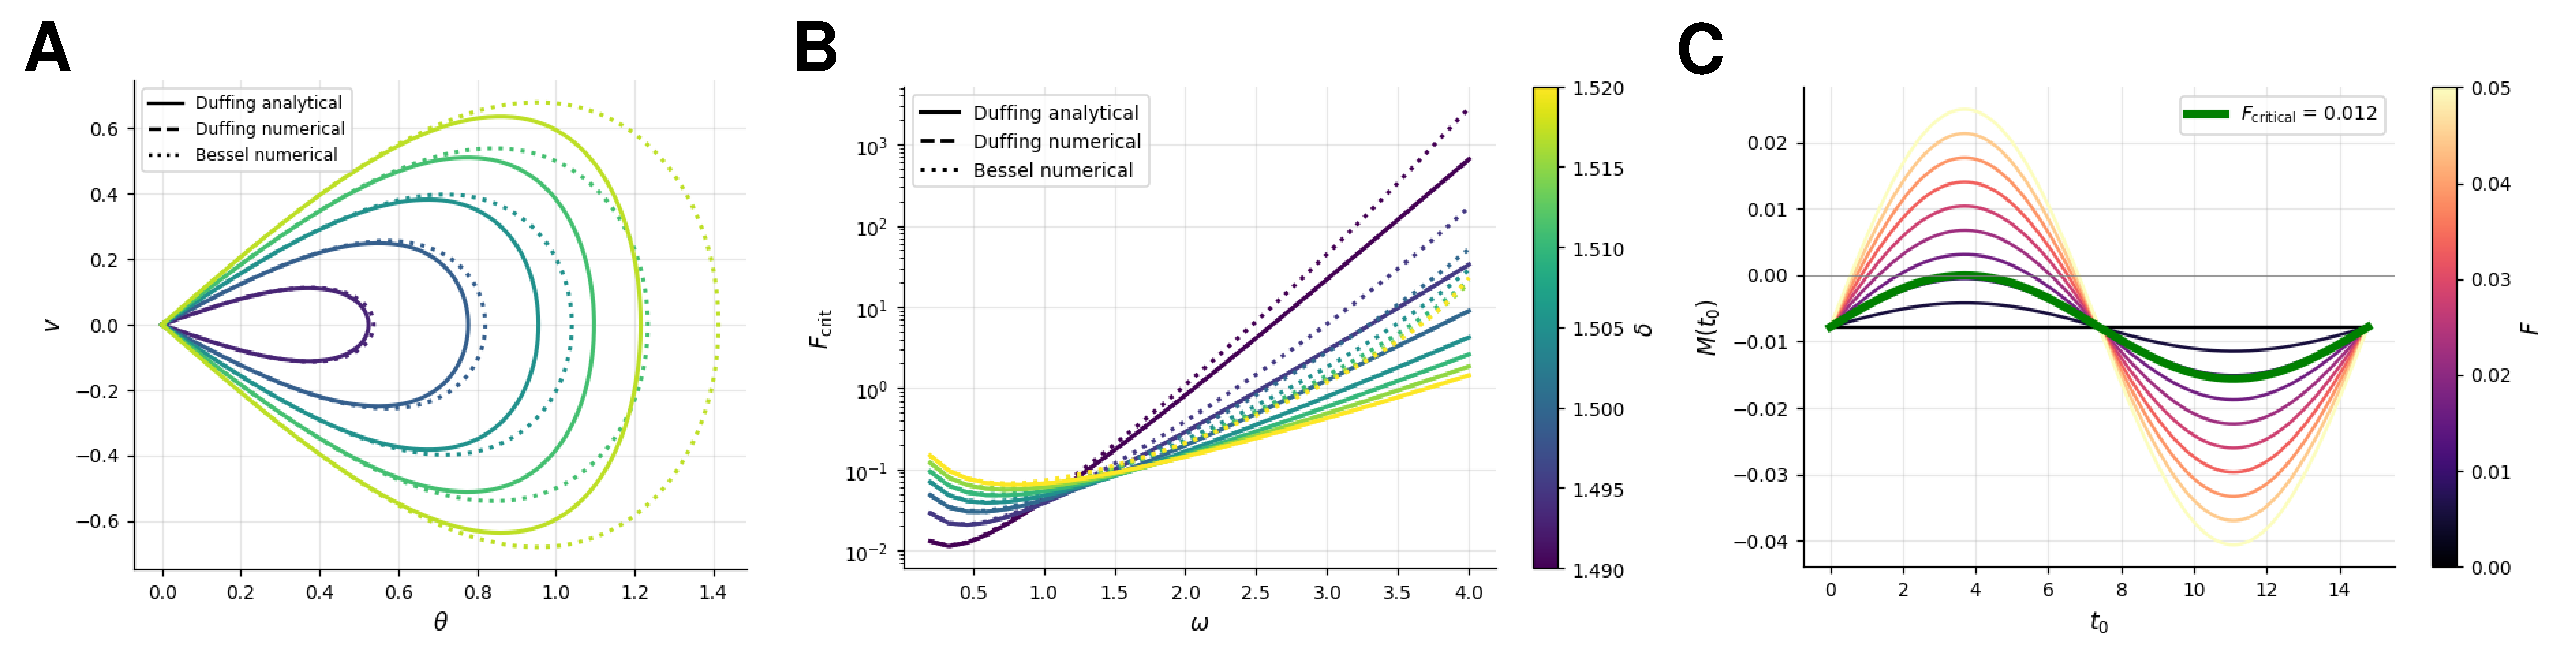
\includegraphics[width=0.85\textwidth]{figures/fig4.pdf}
  \caption{Melnikov analysis comparing the Duffing and Bessel homoclinics.  (A)
  Phase-plane overlay of the three homoclinic orbits across $\delta \in [1.49,
  1.52]$.  (B) $F_{\mathrm{crit}}(\omega)$ on a log scale; the Bessel curve
  (dotted) peels above the Duffing at high $\omega$.  (C) Melnikov function
  $M(t_0)$ vs.\ $t_0$ for $F$ swept from $0$ to $0.05$; bold green curve marks
  $F = F_{\mathrm{crit}}$.}
\end{figure}

In the next sessions, we fix the parameters $\kappa = 1.0$, $\delta = 1.49$ (well inside the bistable regime of Figure 2), and $\gamma = 0.1$. This yields $A \approx 0.18$, $B \approx 1.31$. We choose the forcing frequency

\begin{equation*}
\omega = \sqrt{A} \approx 0.43,
\end{equation*}

which is the convention used in Guckenheimer \& Holmes \cite{guckenheimer1983} for the canonical twin-well Duffing. This $\omega$ is close to (though not exactly at) the forcing-minimizing optimum. Along Figure 4B, these parameters yield very similar homoclinics and $F_{\text{crit}}$ between the Bessel and Duffing systems.

Panel C illustrates the structure of the Melnikov function itself at the chosen parameters, as $F$ is swept from $0$ to $0.05$. At $F = 0$, $M(t_0) = -\gamma D < 0$ is a horizontal line --- the manifolds are separated by a uniform energy gap and no intersection occurs. As $F$ increases, the sinusoidal contribution grows in amplitude. The critical curve $F = F_{\text{crit}} \approx 0.012$ (bold green) is exactly the value at which $M(t_0)$ first touches zero --- quadratically, at a single phase. For $F > F_{\text{crit}}$, $M(t_0)$ has two simple zeros per forcing period, both crossing $M = 0$ transversally; the manifold intersections are transverse and the Smale-Birkhoff conclusion holds across the entire $F > F_{\text{crit}}$ regime shown. The Melnikov criterion is thus a \textit{lower bound} on the existence of horseshoe chaos.

\subsection{Numerical verification near the homoclinic-resonance frequency}

We then perform a loose grid search over the forcing amplitude. Substituting our chosen parameters into (30) gives $F_{\text{crit}} \approx 0.012$, and we grid

\begin{equation*}
F \in \{1.0,\, 1.5,\, 2.0,\, 2.5,\, 3.0\} \times F_{\text{crit}},
\end{equation*}

integrating (20) for the reduced Duffing model and for the 12-neuron discrete circuit model from initial conditions in the right well ($\theta_0 = \sqrt{A/B}, v_0 = 0$). We should note that the 12-neuron model, as illustrated previously in the shape of $U(\theta)$, yields a nearly identical control law as the Bessel limit. We checked (not shown here) that the empirical behaviors under perturbation are also very similar. For each run we discard the first 200 forcing periods as transient and record the next 1000 stroboscopic samples $(\theta_n, v_n) = (\theta(t_n), v(t_n))$ at $t_n = 2\pi n/\omega$. We then sweep $F$ over a denser grid to construct the Poincaré bifurcation diagram $\theta_n$ vs $F$.

\textbf{Figure 5} presents three rows: (A) reduced Duffing, (B) 12-neuron full circuit at $\delta = 1.49$ (the bistable regime), and (C) 6-neuron full circuit at the same bistable regime, but as previously shown only has a single attractor (hence belonging to the monostable regime). Each row contains four panels: (i) stroboscopic Poincaré sections at the five grid-search values of $F$; (ii) the Poincaré bifurcation diagram on a narrow zoom $F \in [0, 0.1]$ revealing the route to chaos; (iii) full phase-space trajectories at the same five $F$ values; (iv) the bifurcation diagram on a wide zoom $F \in [0, 10]$ exposing the regime of large forcing studied in §4.4.

\begin{figure}[htbp]
\centering
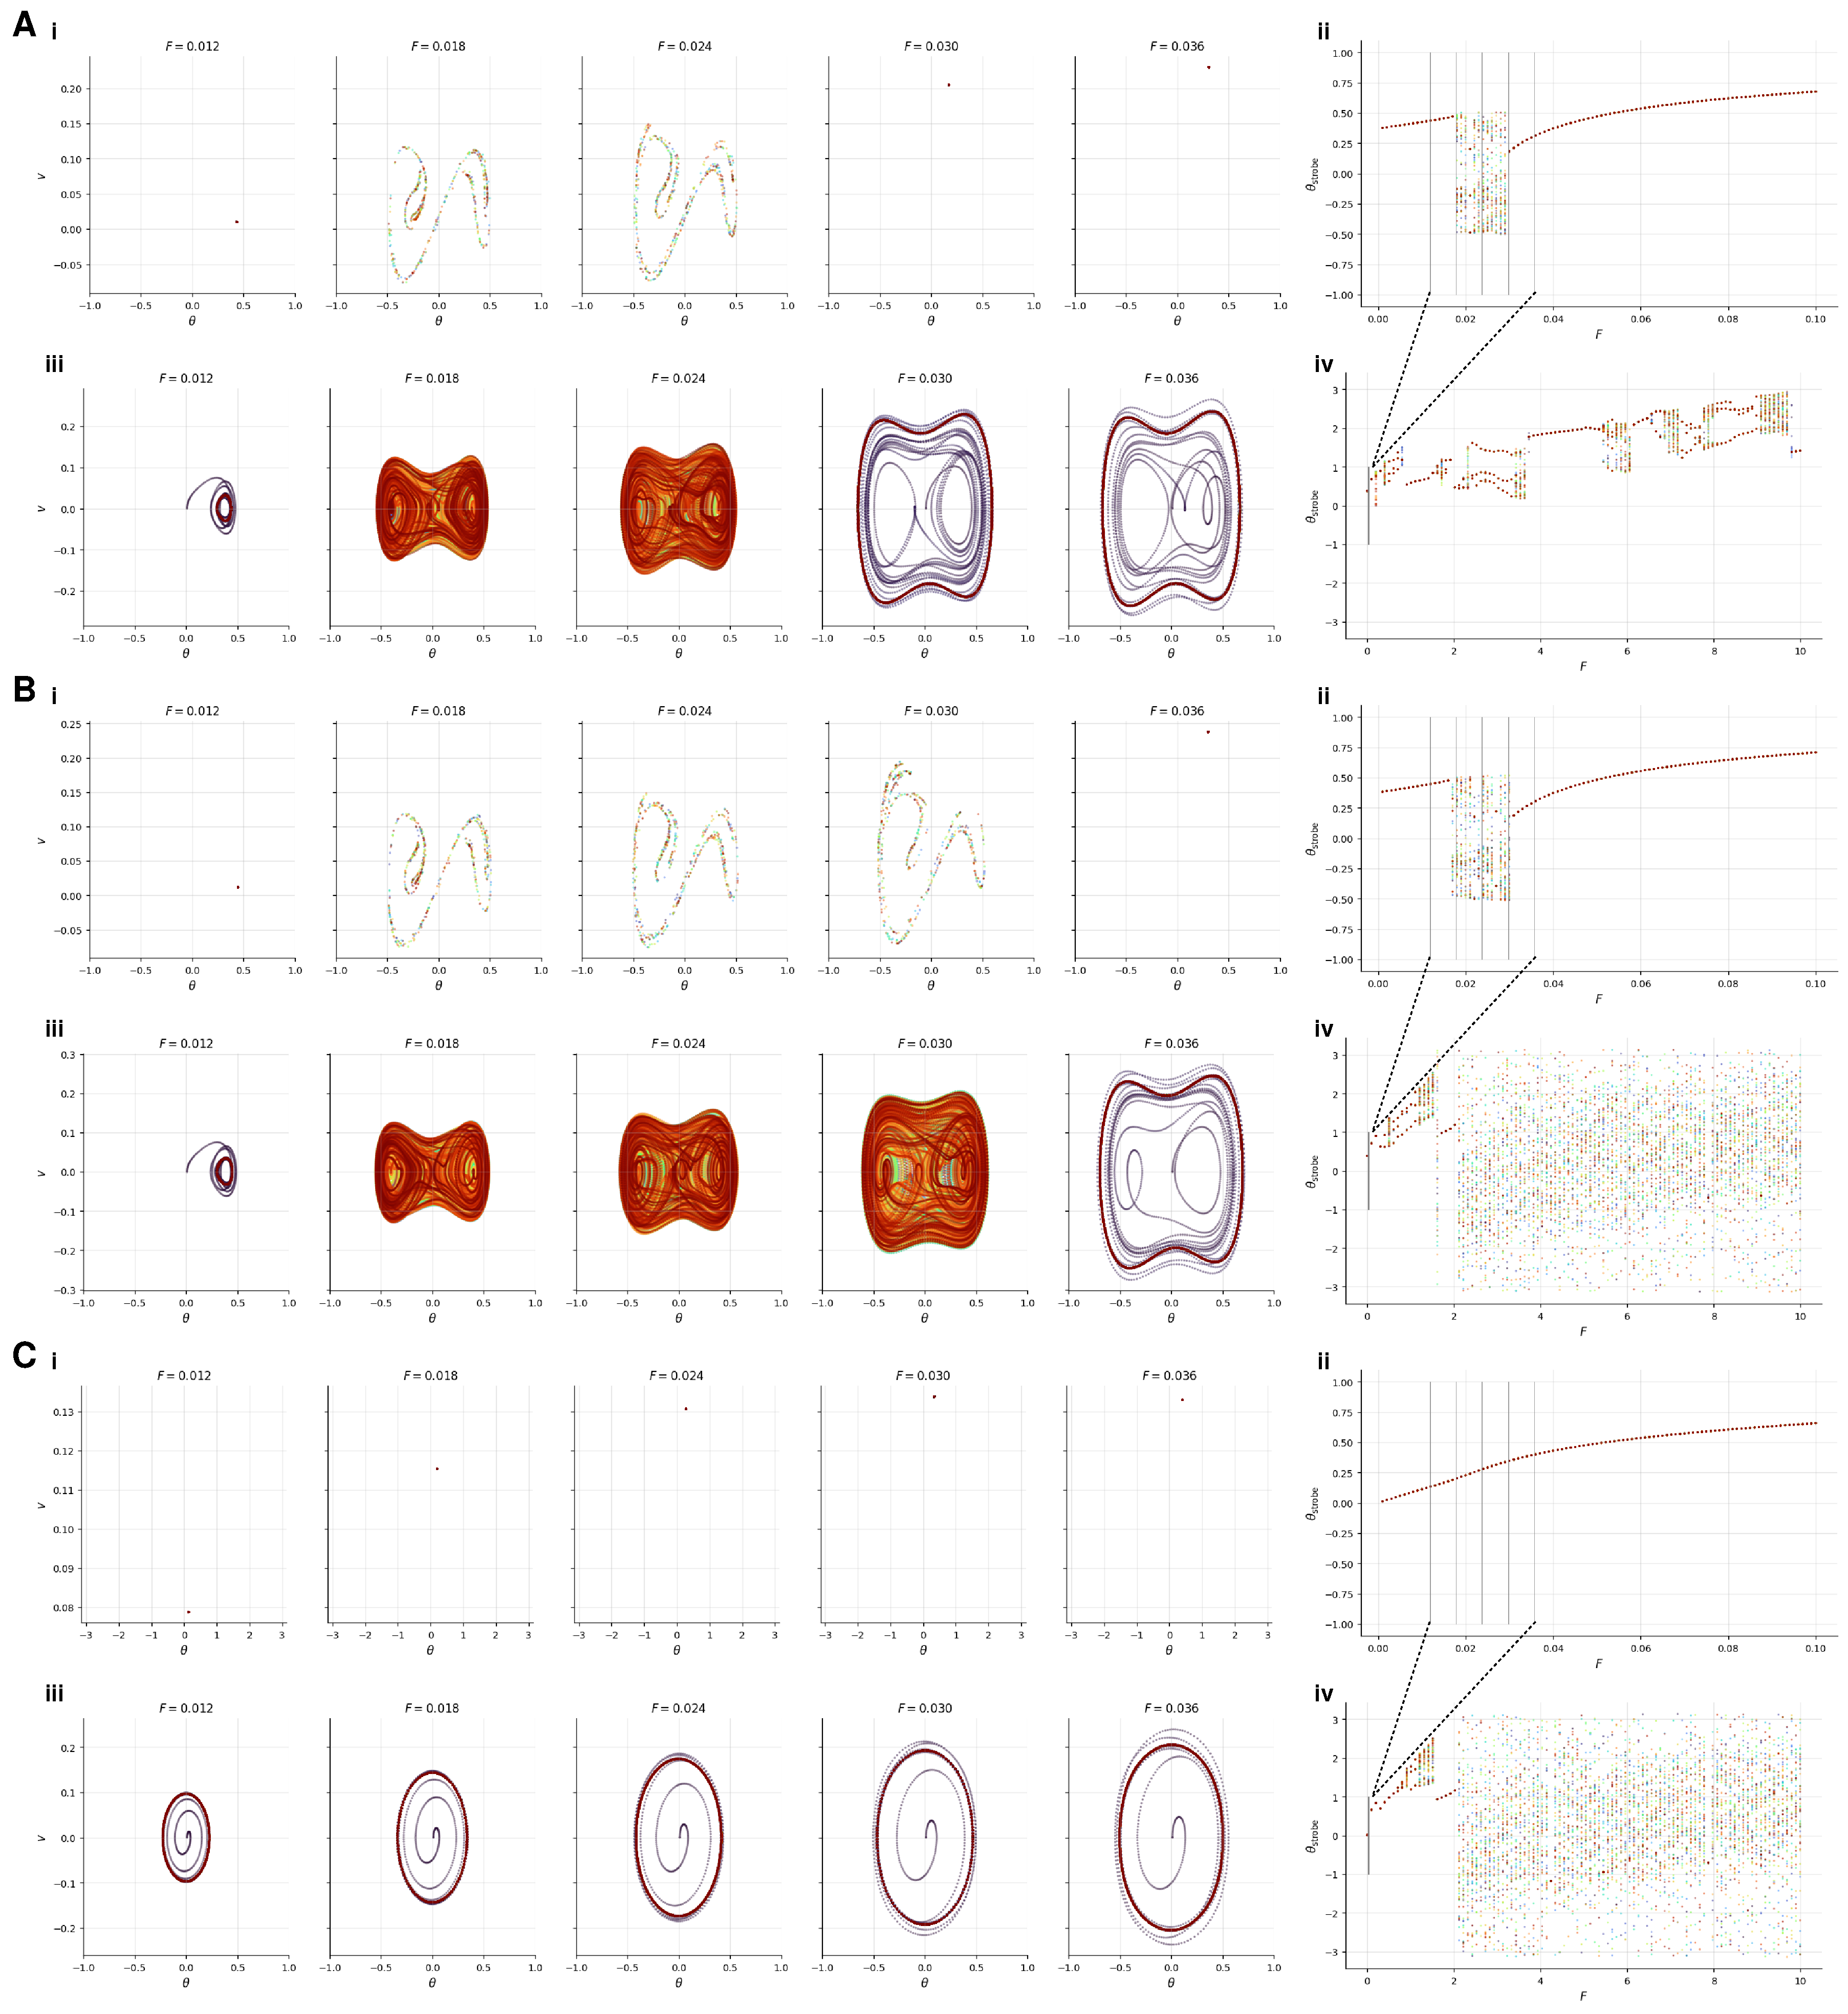
\includegraphics[width=\textwidth]{figures/fig5.pdf}
\caption{Poincaré sections, bifurcation diagrams, and phase-space trajectories
  for (A) the reduced Duffing model, (B) the 12-neuron circuit in the bistable
  regime ($\delta = 1.49$), and (C) the 6-neuron circuit in the monostable
  regime.  Each row contains panels (i) stroboscopic Poincaré sections at five
  forcing amplitudes; (ii) narrow-zoom Poincaré bifurcation diagram; (iii)
  phase-space trajectories; (iv) wide-zoom bifurcation diagram.}
\end{figure}

Across both the reduced Duffing (row A) and the 12-neuron circuit (row B), we observe the same qualitative structure. At $F = F_{\text{crit}}$ (column 1 of panels i and iii) the attractor remains a period-1 orbit confined to the right well. By $F \approx 1.5\,F_{\text{crit}}$ (column 2) the periodic orbit has lost stability and the trajectory has filled out a strange attractor that visibly explores both wells, crossing the unperturbed separatrix infinitely often. The bifurcation diagrams in panel (ii) show the characteristic interleaving of chaotic bands and narrow periodic windows in this $F$ range. By $F \approx 2.5\text{--}3\,F_{\text{crit}}$ (columns 4--5) the trajectory has re-collapsed onto a periodic orbit of large amplitude, encircling both centers.

The factor-of-$1.5$ gap between the Melnikov threshold and the visible onset of chaos may be due to that the Melnikov threshold only proves the existence of the horseshoe but does not distinguish if the invariant set is an attractor or not. We leave detailed analysis of the stability type of the horseshoe for future work. Nonetheless, the agreement between the reduced model (A) and the 12-neuron circuit (B) is quantitatively close, with the chaos band of (B) shifted slightly to higher $F$. This validates the Duffing reduction as a faithful predictor of chaos onset in the biological circuit, at least in this parameter regime.

Row (C), the 6 neuron case where the system sits below the pitchfork curve, provides a useful control: here the unforced system has a single stable fixed point and no homoclinic orbit, so the Melnikov machinery does not apply. Correspondingly, the trajectories in panel (C-iii) remain periodic across the entire grid --- no chaos emerges at these forcing amplitudes. The strange attractor of (A) and (B) is genuinely a consequence of the double-well structure produced by the pitchfork bifurcation.

For the limited scope of the present project, we restrict attention to an initial condition in the right well throughout. However, we expect similar behavior for other nearby initializations in the case of strange attractors.

\subsection{A second chaotic regime: phase-slipping and the pendulum analogy}

The wide-zoom bifurcation diagrams in panels (A-iv) and (B-iv) of Figure 5, together with the snapshots in \textbf{Figure 6}, reveal a striking divergence between the reduced and full systems at large forcing amplitudes ($F \gtrsim 2$, two orders of magnitude above $F_{\text{crit}}$).

In the reduced Duffing model (Figure 6A), increasing $F$ eventually drives the trajectory out of the chaotic regime into a large-amplitude periodic orbit that encircles both wells. The Poincaré section in this regime is a small number of isolated points (Figure 6A-i, $F = 2.25$ through $3.0$) and the phase-space trajectory (Figure 6A-ii) is a smooth closed curve oscillating between $\theta \approx \pm 3$. This is the ``global'' periodic attractor familiar from the standard forced Duffing oscillator.

The full circuit (Figure 6B) behaves qualitatively differently in the same parameter range. Rather than settling onto a closed periodic orbit, the trajectory undergoes \textbf{phase slipping}: $\theta$ executes net rotations around the cylinder $S^1$ rather than remaining bounded. The Poincaré sections (Figure 6B-i) are wide diffuse clouds extending across the full range of $\theta$ and reaching velocities $|v| \sim 10$, an order of magnitude larger than in the Duffing-type chaos of Figure 5. The phase trajectories, as observed in Figure 6B-ii, wrap repeatedly around the cylinder.

\begin{figure}[htbp]
\centering
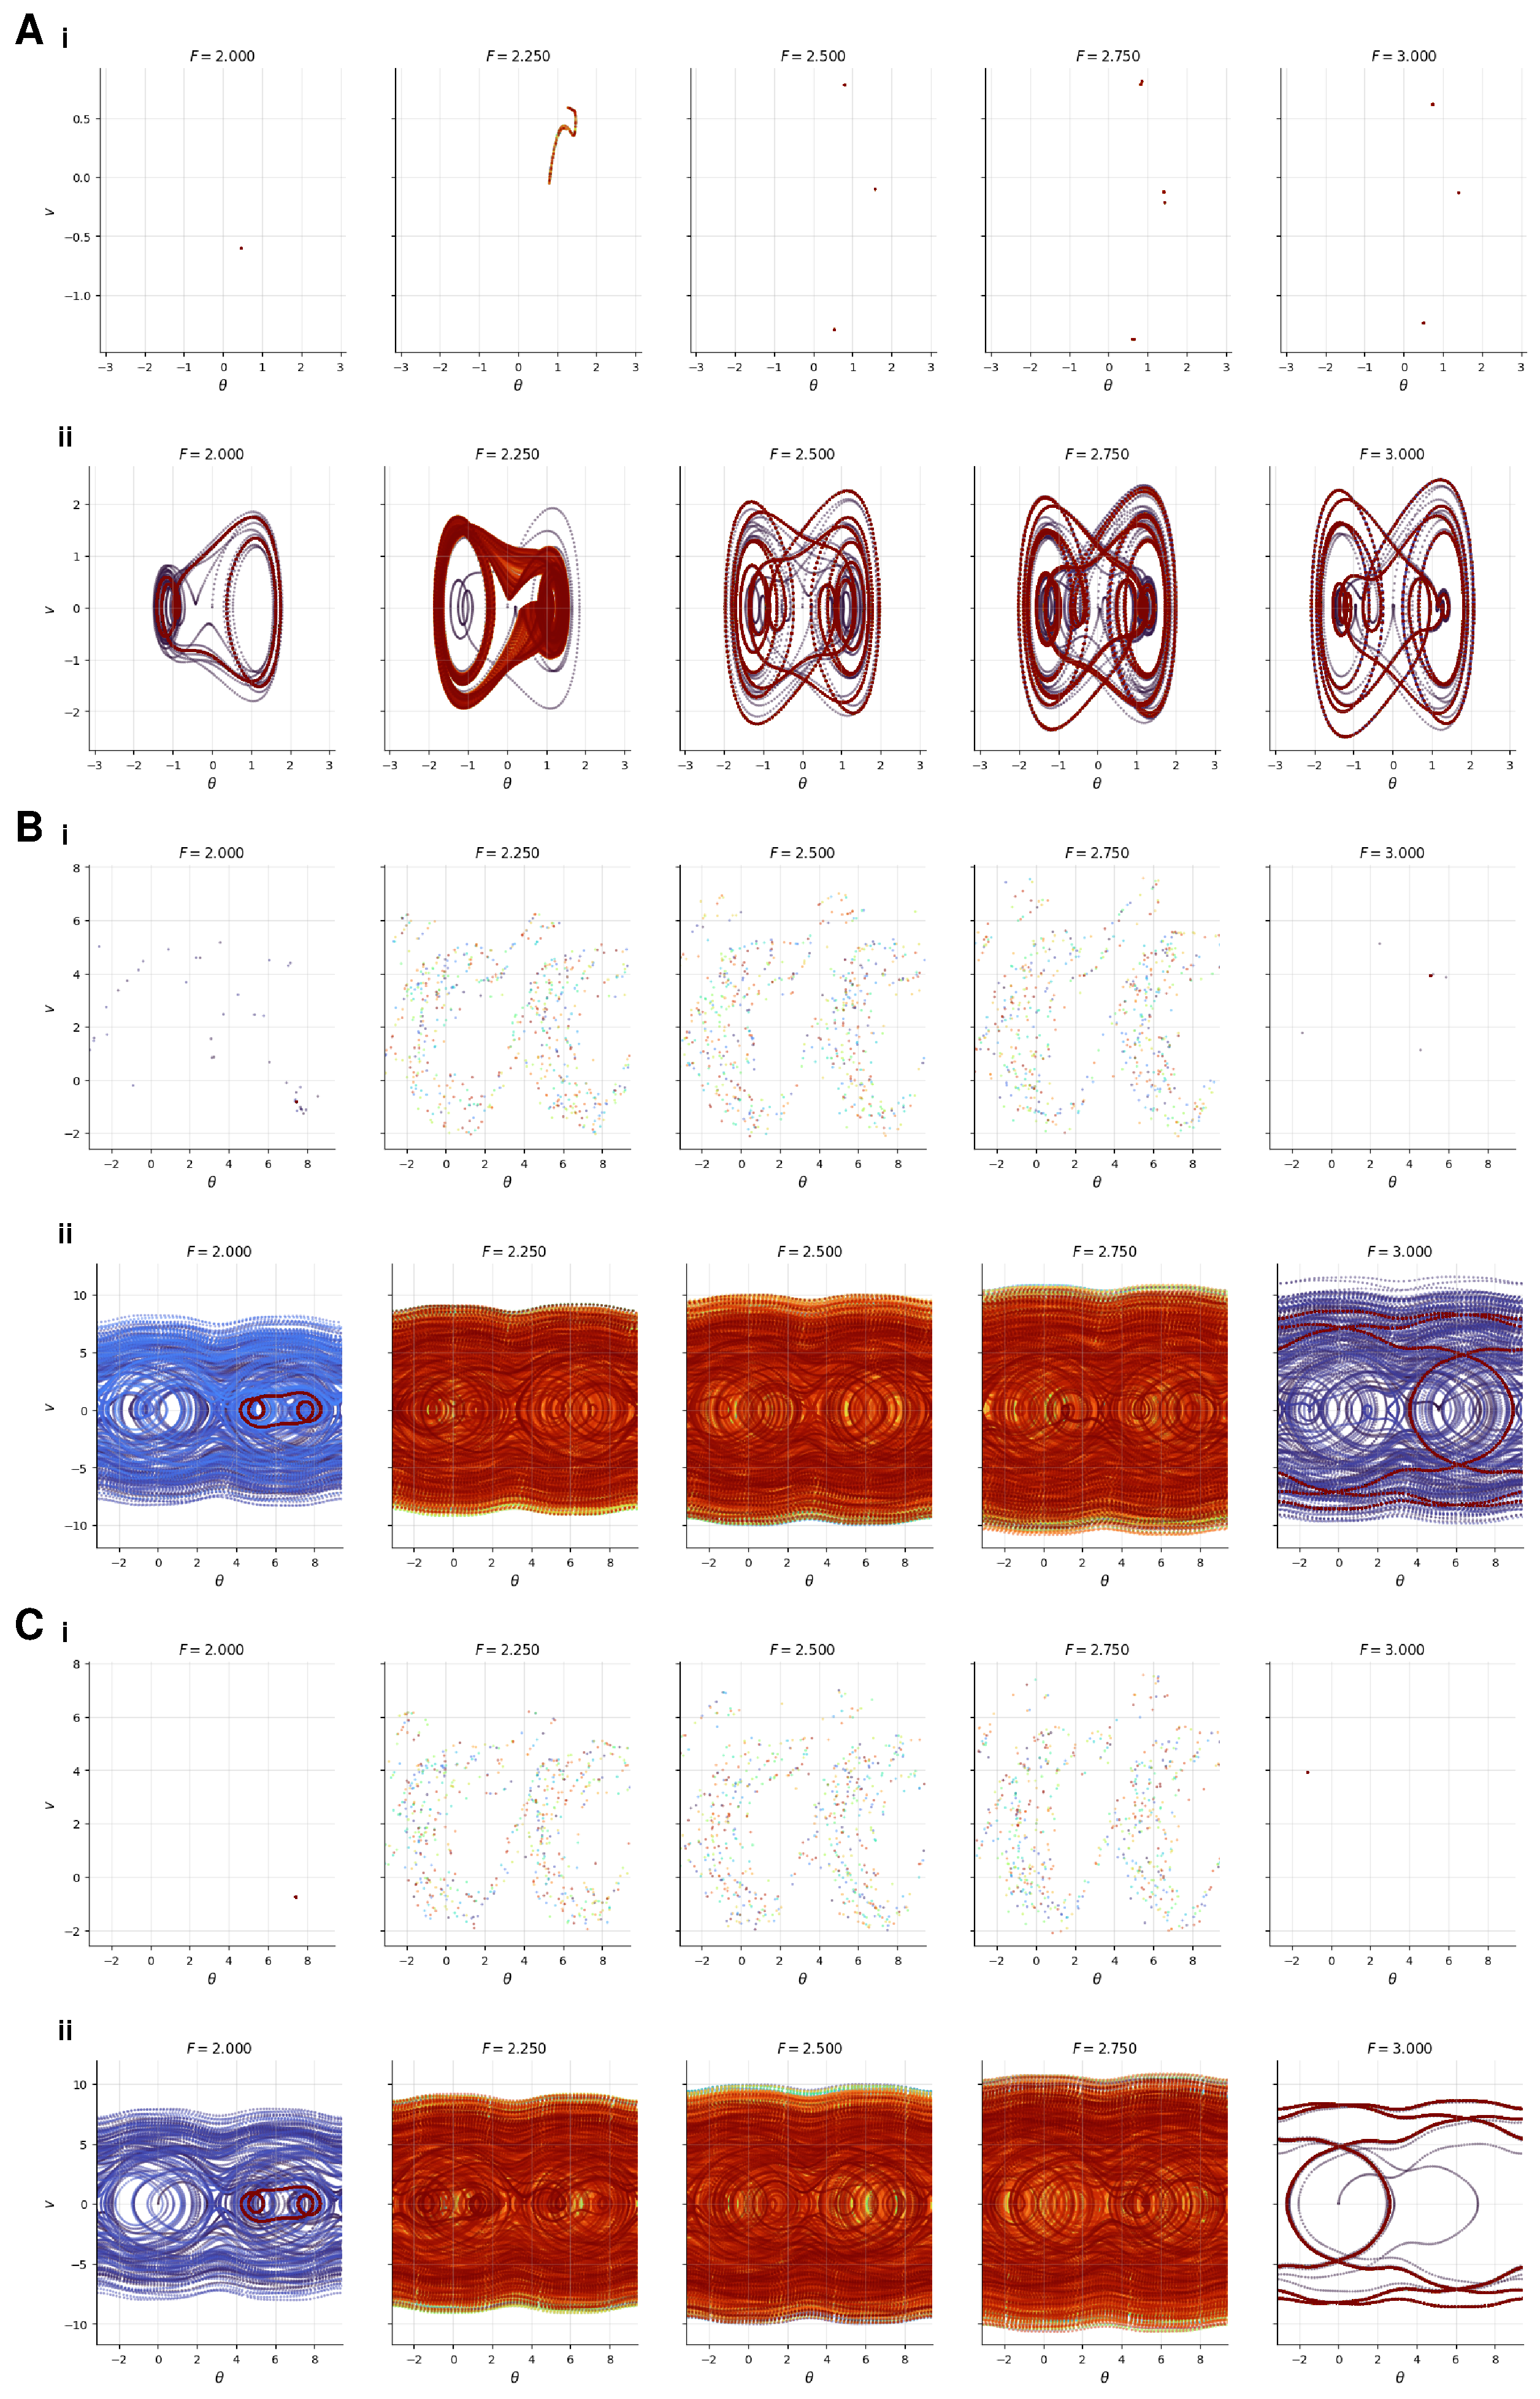
\includegraphics[width=0.75\textwidth]{figures/fig6.pdf}
  \caption{Large-amplitude forcing regime for (A) the reduced Duffing model,
  (B) the full circuit in the bistable regime, and (C) the full circuit in the
  monostable regime.  Each case shows (i) Poincaré sections and (ii) phase-space
  trajectories.  Rows B and C both exhibit phase-slipping chaos absent from the
  Duffing reduction.}
\end{figure}

This phenomenon is invisible to the Duffing reduction, but it is naturally understood through analogy with the forced damped pendulum,

\begin{equation*}
\ddot\varphi + \gamma\dot\varphi + \sin\varphi = F\cos\omega t,
\end{equation*}

which has been studied extensively as a model system for chaos on the phase cylinder \cite{guckenheimer1983}. The pendulum has two equivalent saddle points at $\varphi = \pm\pi$ (identified on $S^1$) connected by two heteroclinic orbits --- the upper and lower branches of the separatrix that bound the regions of librating versus rotating motion. Under periodic forcing, transverse intersections of the stable and unstable manifolds of these heteroclinic connections generate a chaotic invariant set on which the trajectory irregularly switches between librating and rotating behavior, with the rotating component manifesting macroscopically as phase slip \cite{guckenheimer1983}.

Our full Bessel system, regardless of the between-goal pitchfork, inherits this pendulum-like structure: the steering drive $U(\theta, \delta)$ vanishes at $\theta = 0$ (the unstable saddle between the two goals, when bistable) and at $\theta = \pm\pi$ (the saddles associated with the anti-midpoint of the two goals; cf. Figure 2 right panel). When the trajectory has enough energy to traverse the global separatrix, it can transit between adjacent saddles, producing phase slipping analogous to the rotating regime of the forced pendulum. The chaotic dynamics of Figure 6B is most naturally described as transverse intersection of the heteroclinic manifolds connecting the $\theta = \pm\pi$ saddles, rather than the homoclinic intersection that governs Figure 5.

A revealing comparison is provided by row C of Figure 6, which uses the same large-$F$ protocol to query the monostable regime, as shown in Figure 5C. In this configuration the cubic reduction predicts no chaos at any $F$ --- there is no double-well structure and no homoclinic orbit. Yet the full system (Figure 6C) still exhibits phase-slipping chaos at large $F$, qualitatively indistinguishable from Figure 6B. This is direct evidence that the second chaotic regime is \textbf{not} a consequence of the goal-induced double well, but of the global $S^1$ structure of the steering drive. The reduced Duffing model is silent on this regime for its local nature: the cubic truncation captures the saddle at $\theta = 0$ but discards the saddles at $\theta = \pm\pi$.

Another round of Melnikov analysis of phase-slipping chaos is conceptually straightforward but operationally involved, and the resulting expression for the chaos threshold would depend on $(\delta, \kappa, \gamma, \omega)$ through circuit-specific integrals analogous to (28). We leave this as a direction for future work. For the present, we content ourselves with the numerical demonstration that two distinct chaotic regimes exist in the steering circuit --- one captured faithfully by the Duffing reduction near $F_{\text{crit}}$, and a second, global regime accessible only through the full Bessel or neural circuit model.

\section{Discussion}

Our analysis has established that the \textit{Drosophila} steering circuit, under the assumption of dual-goal von Mises representations, generates a local cubic normal form whose forced version supports two distinct chaotic regimes: a local, dual-goal-induced homoclinic chaos near the Melnikov threshold, and a global, pendulum-like heteroclinic chaos at larger forcing. Whether either of these regimes is realized in the behaving fly and which natural perturbations could induce them depend on several factors that this work does not fully resolve. We close by outlining what is needed to bridge the theoretical analysis to biological validation.

\subsection{Inertia, friction, and the realized $F(\omega)$ surface}

The Melnikov criterion (31) gives $F_{\text{crit}}$ as a function of the dimensionless parameters $A, B, \gamma, \omega$, but the mapping back to physical forcing amplitudes and frequencies depends sensitively on the body's rotational inertia $I$ and frictional drag $\gamma_{\text{phys}}$. In our units (setting $I = 1$ rescales time by a natural scale $\sqrt{I/T_0}$ with $T_0$ a reference torque), the dimensionless $\omega$ corresponds to a physical frequency $\omega_{\text{phys}} = \omega\sqrt{T_0/I}$. The dual-goal chaos predicted near $F_{\text{crit}} \sim 0.01$ in our units may correspond to physical torque perturbations within or beyond the range that natural sensory streams can deliver, depending on these calibration factors.

This caveat applies most stringently to the local chaos of §4.3, which lives in a narrow window of $F$ and $\omega$ (Figure 5) --- the homoclinic resonance is sharp, and a mismatch between the natural frequencies of biological perturbations and the system's $\omega \approx 0.76\sqrt{A}$ may suppress visible chaos. The phase-slipping chaos of §4.4, by contrast, is observed across two orders of magnitude in $F$ and is more robust to frequency choice. If the goal is to observe chaotic steering experimentally --- for instance, by driving the central complex with optogenetic perturbations or visual stimulation of a chosen frequency --- the phase-slipping regime is more accessible, requiring only that the forcing amplitude be sufficiently large to push the system into the rotational regime of the phase cylinder.

\subsection{The Melnikov bound is approximate}

The factor of approximately 1.5 between the Melnikov threshold and the observable onset of chaos in §4.3 may be attributed to two sources. First, the Melnikov function is leading-order in the perturbation parameter $\epsilon$, which may deviate from the true threshold to the horse-shoe by $\mathcal{O}(\epsilon^{2})$. Second, the horseshoe born at the Melnikov threshold is not necessarily an attractor, so its existence does not by itself imply observable chaos. We did not run dedicated numerical experiments to disentangle these two contributions.

Empirically, the gap is likely to be a complicated function of $\omega$. At high $\omega$, $F_{\text{crit}}$ grows exponentially through the $\cosh$ factor and the perturbation parameter $F/\sqrt{2A^3/B}$ leaves the small-$\epsilon$ regime entirely, so (31) ceases to be reliable as a quantitative predictor --- the relevant chaos onset must be determined numerically, and the ratio $F_{\text{actual}}/F_{\text{Melnikov}}$ likely varies non-monotonically with $\omega$. Mapping this gap numerically across the $(\omega, \delta)$ plane is a natural next step before attempting to predict experimental parameters of chaos onset.

Further, the deterministic forced Duffing analysis we have presented neglects any stochasticity, which is unrealistic in biological systems. We leave further explorations of this topic to future studies of dynamical systems.

\subsection{Representation of dual goals}

Our entire analysis rests on the specific representation of two simultaneous goals as a superposition of two von Mises bumps with equal amplitude and concentration. This is a modeling choice --- biologically, the goal representation could also be implemented as a \textit{temporal switching} between two single-goal bumps (winner-takes-all dynamics with stochastic transitions), or as a deformed single bump shifted toward the resultant direction. The von Mises superposition is the only one of these that genuinely yields bistability in the steering drive: as established in §1, single-bump representations (whether static or time-averaged) collapse to unimodal steering profiles and cannot generate a pitchfork bifurcation. The phase-slipping chaos of §4.4, however, is independent of dual-goal structure and would persist under any of these representational schemes, since it arises from the global $S^1$ topology of the steering drive rather than from the goal-induced double well.

\subsection{The role of PFL2 and the nonlinearity choice}

Finally, it is worth noting that the full circuit model (with PFL2 cells and the indirect pathway) yields surprisingly similar $U(\theta)$ profiles to the PFL3-only reduction (Figure 1), suggesting a redundancy of PFL2 in our model that contradicts experimental observations of PFL2's role \cite{westeinde2024}. This inconsistency may result from our choice of quadratic nonlinearity $f(x) = x^2$ rather than the ELU used in Westeinde et al. \cite{westeinde2024}. The ELU's asymmetric rectification could act as a gating mechanism, selectively activating subpopulations of control neurons in a manner that the quadratic model cannot capture. A more rigorous analysis of the complete circuit model, including more biologically informed modelling choices, would clarify whether PFL2 plays a structural role in shaping the chaos thresholds of the steering system. Combined with the switching-bump representations above, this would form a fuller theoretical picture of how the central complex's neural architecture supports robust, multi-goal navigation in the face of perturbations.

\section*{Notation and conventions}

For ease of cross-reference:

\begin{itemize}
\item $\theta$: fly's heading.
\item $\delta$: half-separation of the two goals (goals at $\pm\delta$).
\item $\phi$: preferred direction of a PFL/goal/heading neuron (integration variable).
\item $\Delta_{PFL3}$: PFL3L heading-input phase shift ($+67.5^\circ$ for L, $-67.5^\circ$ for R, by convention here).
\item $\kappa_{\text{heading}}, \kappa_{\text{goal}}$: von Mises concentrations of heading and goal bumps. Often taken equal to $\kappa$.
\item $\kappa(a, b) = \sqrt{\kappa_h^2 + \kappa_g^2 + 2\kappa_h\kappa_g\cos(a-b)}$: effective concentration after phasor sum.
\item $\mu(a, b)$: effective phase (drops out after $\phi$ integration).
\item $S, A$: synaptic gain on heading and goal inputs (both positive, set by biology).
\item $f(x) = x^2$: quadratic nonlinearity (conjunctive tuning).
\item $U(\theta, \delta)$: total steering drive, $G_{PFL3} - G_{PFL3R}$.
\end{itemize}

\bibliographystyle{plain}
\bibliography{steering}

\printbibliography
\end{document}
